\documentclass[aps,
                pra,  
                a4paper, 
                amsmath, 
                amssymb, 
                preprint,
                tightenlines,  
                amsfonts,
                nofootinbib,
                %onecolumn,
            ]{revtex4-2}
\usepackage[utf8]{inputenc}
\usepackage{graphicx}
\usepackage[rightcaption]{sidecap}

\begin{document}

%Title
\title{PHYS4420 Assignment:\\Analysis of x-ray sources within the $\omega$-Centauri globular cluster}

%Authors and Info
\author{Joseph Hocking}
\email{22876965@student.uwa.edu.au}
\noaffiliation

%Compilation Date
\date{\today}

\begin{abstract}
    TODO
\end{abstract}

\maketitle

\section{Introduction}
\subsection{What is the $\omega$-Centauri Globular Cluster?}
Globular clusters are broadly spherical group of stars on the order of $\sim10^5-10^6$ objects. The globular cluster NGC 5139, more commonly referred to as $\omega$-Centauri (from here on $\omega$ Cen) is a well known historical example of a globular cluster. It was first identified by Greek astronomers, who in the 2nd century AD wrongly classified it as a star. It wasn't until Edmond Halley in 1677, taking advantage of the recent invention of the telescope, discovered that it was in fact a non-stellar object, however it took a further 150 years before James Dunlop classified it as a globular cluster. It is unique in that it is the largest globular cluster known within the Milky Way, with a radius of $86\pm6$ly and an estimated mass of $(4.05\pm0.1)\times10^6M_{\odot}$, which, along with other evidence for an intermediate mass black hole in its core, leads some to argue that it may in fact be a remnant of a dwarf galaxy, swallowed by the much larger Milky Way.
\par
The main mechanism of internal cluster dynamical evolution is due to gravitational iteraction between bodies. Statiscally, one may derive an approximate rule for the \textit{relaxation time} of a globular cluster as follows:
\begin{equation}
    t_{relax}\approx\frac{0.1N}{\log{N}}t_{cross}
\end{equation}
Where $N$ is the number of stars in the cluster, and $t_{cross}$ is the crossing time of stars within the cluster. For the $\omega$ Cen cluster, the half mass relaxation time has been found to be relatively long, at $t_{relax}\approx 10Gyr$. This is significant as the cluster has an estimated age of $\sim 12Gyrs$, thus many of the dynamics within the clusters are similar to those that would occur just after formation. One may observe the effect of this relaxation time by examining the radial distribution (or rather independence) of mass-light ratio, that is, there is broadly an even distribution of high and low mass stars. Whereas in clusters that have evolved over several relation times, the high mass stars tend to migrate towards the center of the cluster.
\par
Another important concept to consider is the effective \textit{negative heat capacity} of a cluster. This is a by-product of the virial theorem within a self gravitating system. Conceptually, as a body in orbit loses energy, its orbit becomes tighter, and thus the body's speed will increase (making it ``hotter"). Additionally, just as in thermodynamical systems, weak gravitational interactions between stars begins to establish an equipartition of kinetic energy. This will ultimately mean stars of higher mass will slow down as they transfer speed to stars of lower mass. Thus a segregation is formed of high mass stars towards the core of the cluster and low mass towards the outside. Because of the negative heat capacity of the cluster, it's core will become denser and denser as time goes on, and relatively quickly resulting in \textit{core collapse}. An easy analogy can be made to the structure of a star, which would undergo gravitational collapse if it were not held at equilibrium by the radiation pressure from nuclear fusion. In the case of globular clusters, the bound energy of binary star systems provide the necessary energy to keep the cluster in equilibrium. When a binary system interacts with outside binaries, there is a chance for one object in the binary to lose energy to the outside object, which through it's negative heat capacity will speed the binary system up, staving off core collapse\footnote{In fact, a single standard mass binary system of two $0.7M_{\odot}$ stars are able to contain more binding energy than the entire cluster they are contained within}. This mechanism is able to extend the time before core collapse to $\sim 10t_{relax}$. It is also interesting to note that observations have showing that insufficient numbers of binaries could be formed through encounters, given the known density of globular cluster cores, and so the majority of these are likely to be primordial binaries (or systems that \textit{formed} as binaries).
\subsection{X-ray sources within Globular Clusters}
\begin{SCfigure}
    \caption{A description of the potential x-ray sources within the globular clusters\cite{Verbunt2006}}
    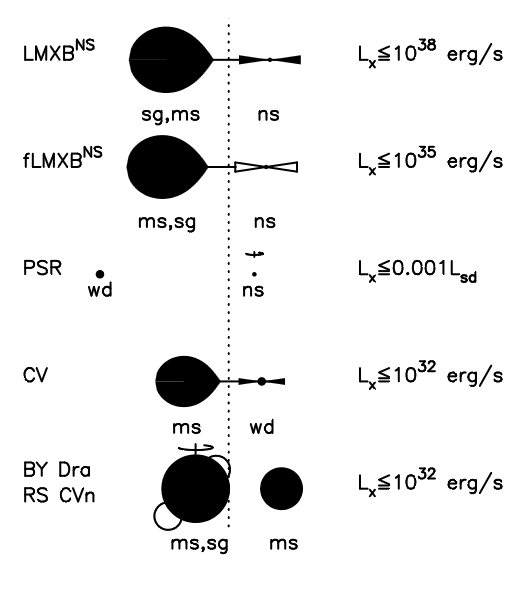
\includegraphics[width=0.4\textwidth]{img/gc-xray-sources.png}
    \label{fig:gc-xray-sources}
\end{SCfigure}
We can split x-ray sources in general into two categories: luminous and low-luminosity. Of the luminous sources with globular cluster, it is considered widely that they are all composed of binary systems of the type shown in Figure \ref{fig:gc-xray-sources}. Additionally the vast majority of low luminosity sources are of these same type or at the very least evolved from binary systems. Given this, and given the importance of binary systems to the stability of globular clusters, studying x-ray sources within globular clusters is crucial to understanding cluster dynamics as a whole. I will now only give a brief discription of each of the x-ray sources given in Figure \ref{fig:gc-xray-sources}, as the relevant source will have a much more detailed explanation in the following sections.

\subsubsection{Low Mass X-Ray Binary (LMXB \& fLMXB)} 
These are binary systems consisting of a compact object\footnote{In Figure \ref{fig:gc-xray-sources}, illustrated as a neutron star (NS-LMXB), but it may also be a black hole (BH-LMXB). However NS-LMXBs occur $\sim 2\times$ as often as BH-LMXBs} and a lower mass companion star typically on the order of $1M_{\odot}$. Large luminosities of x-ray's are emitted when the companion star moves within the ROche lobe of the compact object, creating an accretion disk from the star's outer layers. It is important to note that most LMXB's are in fact transient as the accretion rate usually experiences periodic variations. 

\newpage
\nocite{*}
\bibliography{references}

\end{document}